%
% File eacl2017.tex
%

\documentclass[11pt]{article}
\usepackage{eacl2017}
\usepackage{times}
\usepackage{url}
\usepackage{latexsym}
\usepackage{times}
\usepackage{url}
\usepackage{amsmath}
\usepackage{breqn}
\usepackage{latexsym}
\usepackage{pgfplotstable}
\usepackage{algorithm2e}
\usepackage{hhline}
\usepackage{multirow}
\usepackage[font=small]{caption}
\usepackage{subcaption}
%\usepackage{hyperref}
\usepackage{color}
\usepackage{lipsum,adjustbox}
\usepackage{tikz}
\usepackage{tikz-dependency}
\usetikzlibrary{shapes,fit,calc,er,positioning,intersections,decorations.shapes,mindmap,trees}
\tikzset{decorate sep/.style 2 args={decorate,decoration={shape backgrounds,shape=circle,
      shape size=#1,shape sep=#2}}}
\setlength{\belowcaptionskip}{-10pt}
\addtolength{\parskip}{-0.5mm}
\addtolength{\textfloatsep}{-2mm}
\newcommand{\oa}[1]{\footnote{\color{red} #1}}
\newcommand{\daniel}[1]{\footnote{\color{blue} #1}}
\newcommand{\com}[1]{}
\newcommand{\secref}[1]{Section~\ref{#1}}
\newcommand{\figref}[1]{Figure~\ref{#1}}
\newcommand{\tabref}[1]{Table~\ref{#1}}
\DeclareMathOperator*{\argmin}{argmin}
\DeclareMathOperator*{\argmax}{argmax}
\SetKwRepeat{Do}{do}{while}
\renewcommand\AlCapFnt{\normalfont\small}
\hyphenation{SemEval}

%\eaclfinalcopy % Uncomment this line for the final submission
%\def\eaclpaperid{***} %  Enter the acl Paper ID here

%\setlength\titlebox{5cm}
% You can expand the titlebox if you need extra space
% to show all the authors. Please do not make the titlebox
% smaller than 5cm (the original size); we will check this
% in the camera-ready version and ask you to change it back.

\newcommand\BibTeX{B{\sc ib}\TeX}

\title{Broad-Coverage Semantic Parsing: A Transition-Based Approach}

\author{Daniel Hershcovich \and Omri Abend \and Ari Rappoport \\
  Institute of Computer Science \\
  Hebrew University of Jerusalem \\
  {\tt \{danielh,oabend,arir\}@cs.huji.ac.il}
}

\date{}

\begin{document}
\maketitle

%%%%%%%%%%%%%%%%%%%%%%%%%%%%%%%%%%%%%%%%%%%%%%%%%%%%%%%%%%%%%%%
%%%%%%%%%%%%%%%%%     Abstract
%%%%%%%%%%%%%%%%%%%%%%%%%%%%%%%%%%%%%%%%%%%%%%%%%%%%%%%%%%%%%%%
\begin{abstract}

Semantic annotation schemes and data sets call for parsers not limited to tree structures,
and many languages require non-projective parsing techniques.
The UCCA semantic scheme contains non-terminal nodes in addition to these properties,
and thus parsing it also requires detecting these nodes, corresponding to abstract semantic units.
We propose two techniques for UCCA parsing: one based on approximation by simpler structures,
and a direct broad-coverage parser. We focus on transition-based methods, and experimentally
demonstrate their effectiveness on the task.
  
\end{abstract}



%%%%%%%%%%%%%%%%%%%%%%%%%%%%%%%%%%%%%%%%%%%%%%%%%%%%%%%%%%%%%%%
\section{Introduction}

Tree-oriented parsing has been in the focus of research for several decades,
recently yielding some impressive results.
However, more general graph structures are necessary for semantic representation,
as has been argued to justify two recent SemEval shared tasks
\cite{oepen2014semeval,oepen2015semeval}.

We focus on anchored meaning representation
(semantic units are inherently aligned to the words and phrases of the text),
and claim that three structural properties must be supported to cover the full range of semantic
structures exhibited by natural language.
The first is \textbf{multiple parents},
representing arguments and relations (semantic units) that are shared between predicates.
For instance, in the sentence
``After graduation, John moved to Paris'', ``John'' is an argument of both ``graduation''
and ``moved'', yielding a DAG structure (\figref{fig:graduation}), rather than a tree.

The second is \textbf{non-terminal nodes} for representing units
comprising more than one word.
While bi-lexical dependencies partially circumvent this requirement, by
representing complex units in terms of their headwords, they fall short
when representing units that have no clear head.
Frequent examples of such constructions include
coordination structures (e.g., ``\textit{John and Mary} went home''; \figref{fig:home}),
some multi-word expressions (e.g., ``The Haves and the \textit{Have Nots}''),
and prepositional phrases.
In these cases, dependency schemes often apply some convention selecting one of the sub-units
as the head, but as different head selections are needed for different purposes,
standardization problems arise \cite{Ivanova2012who}.
For example, selecting the preposition to head prepositional phrases yields better
parsing results \cite{Schwartz:12}, while the head noun is more useful for
information extraction.

Third, semantic units may be \textbf{discontinuous}. For instance, in
``John \textit{gave} everything \textit{up}''
(\figref{fig:gave}), the phrasal verb ``gave ... up'' forms a single semantic unit.
Discontinuities are also pervasive with other multi-word
expressions \cite{schneider2014discriminative}.

\begin{figure}[t]
  \begin{subfigure}[t]{.9\columnwidth}
  \parbox{.1\columnwidth}{\caption{}\label{fig:graduation}}
  \parbox{.8\columnwidth}{
  \scalebox{.9}{
  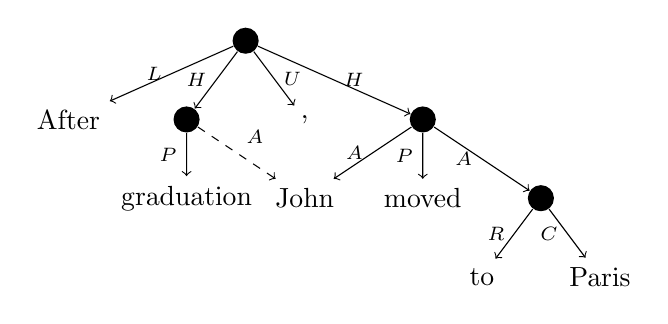
\begin{tikzpicture}[level distance=10mm, ->]
    \node (ROOT) [fill=black, circle] {}
      child {node (After) {After} edge from parent node[left] {\scriptsize $L$}}
      child {node (graduation) [fill=black, circle] {}
      {
        child {node {graduation} edge from parent node[left] {\scriptsize $P$}}
      } edge from parent node[left] {\scriptsize $H$} }
      child {node {,} edge from parent node[right] {\scriptsize $U$}}
      child {node (moved) [fill=black, circle] {}
      {
        child {node (John) {John} edge from parent node[left] {\scriptsize $A$}}
        child {node {moved} edge from parent node[left] {\scriptsize $P$}}
        child {node [fill=black, circle] {}
        {
          child {node {to} edge from parent node[left] {\scriptsize $R$}}
          child {node {Paris} edge from parent node[left] {\scriptsize $C$}}
        } edge from parent node[left] {\scriptsize $A$} }
      } edge from parent node[right] {\scriptsize $H$} }
      ;
    \draw[dashed,->] (graduation) to node [auto] {\scriptsize $A$} (John);
  \end{tikzpicture}
  }}
  \end{subfigure}
  \begin{subfigure}[t]{.9\columnwidth}
  \parbox{.1\columnwidth}{\caption{}\label{fig:home}}
  \hspace{.1\columnwidth}
  \parbox{.7\columnwidth}{
  \scalebox{.9}{
  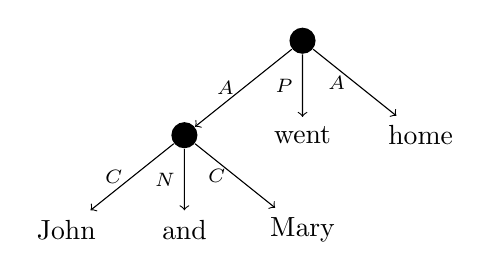
\begin{tikzpicture}[level distance=12mm, ->,
      every node/.append style={midway}]
    \node (ROOT) [fill=black, circle] {}
      child {node [fill=black, circle] {}
      {
        child {node {John} edge from parent node[left] {\scriptsize $C$}}
        child {node {and} edge from parent node[left] {\scriptsize $N$}}
        child {node {Mary} edge from parent node[left] {\scriptsize $C$}}
      } edge from parent node[left] {\scriptsize $A$} }
      child {node {went} edge from parent node[left] {\scriptsize $P$}}
      child {node {home} edge from parent node[left] {\scriptsize $A$}}
      ;
  \end{tikzpicture}
  }}
  \end{subfigure}
  \begin{subfigure}[t]{.9\columnwidth}
  \parbox{.1\columnwidth}{\caption{}\label{fig:gave}}
  \hspace{.25\columnwidth}
  \parbox{.55\columnwidth}{
  \scalebox{.9}{
  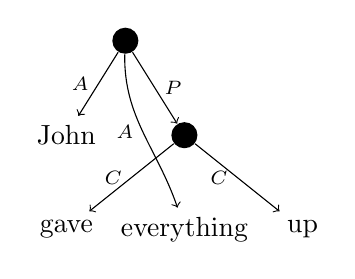
\begin{tikzpicture}[level distance=12mm, ->,
      every node/.append style={midway}]
    \node (ROOT) [fill=black, circle] {}
      child {node {John} edge from parent node[left] {\scriptsize $A$}}
      child {node [fill=black, circle] {}
      {
      	child {node {gave} edge from parent node[left] {\scriptsize $C$}}
      	child {node (everything) {everything} edge from parent[white]}
      	child {node {up} edge from parent node[left] {\scriptsize $C$}}
      } edge from parent node[right] {\scriptsize $P$} }
      ;
    \draw[bend right,->] (ROOT) to[out=-20, in=180] node [left] {\scriptsize $A$} (everything);
  \end{tikzpicture}
  }}
  \end{subfigure}
  \caption{\label{fig:examples}
    Semantic representation of the three structural properties
    required for BSS, according to the UCCA scheme. (\subref{fig:graduation}) includes a remote edge (dashed),
    resulting in ``John'' having two parents. % and a linkage relation (gray node and its outgoing edges).
    (\subref{fig:home}) includes a coordination construction (``John and Mary'').
    (\subref{fig:gave}) includes a discontinuous unit (``gave ... up'').
    Legend: $P$ -- a Scene's main relation, $A$ -- participant,
    $L$ -- inter-scene linker, $H$ -- linked Scene, $C$ -- center,
    $R$ -- relator, $N$ -- connector, $U$ -- punctuation, $F$ -- function unit.
    Pre-terminal nodes are omitted for brevity.
  }
\end{figure}

We experiment with the UCCA scheme and annotated corpora \cite{abend2013universal},
which exhibit all three properties.
We focus on transition-based methods---a natural starting point for UCCA parsing,
given their recently proven fitness for similar tasks, including syntactic dependency parsing
\cite{dyer2015transition,andor2016globally,kiperwasser2016simple},
discontinuous syntactic constituency parsing
\cite{maier-lichte:2016:DiscoNLP} and AMR parsing
\cite{wang-EtAl:2016:SemEval}.

\daniel{update}
We pursue two complementary parsing strategies.
First, we assess the ability of existing technology to tackle the task,
by developing conversion protocols between UCCA structures and two related formalisms:
dependency and constituency trees.
As these formalisms are more restrictive than BSS, the conversion
is necessarily lossy. Nonetheless, we find that it is effective
in practice (\secref{sec:conversion_approach}).
Second, we present a novel transition-based broad-coverage parser,
(\textsc{bsp}; \secref{sec:direct_approach})
supporting multiple parents, non-terminal nodes and discontinuous units,
based on extending existing transition-based parsers
with new transitions and features.

The results suggest concrete paths for further improvement.
All converters and parsers will be made publicly available upon publication.


%%%%%%%%%%%%%%%%%%%%%%%%%%%%%%%%%%%%%%%%%%%%%%%%%%%%%%%%%%%%%%%

\section{Related Work}\label{sec:related_work}
While earlier work on anchored semantic parsing has mostly concentrated on shallow semantic analysis,
focusing on semantic role labeling of verbal argument structures,
the focus has recently shifted to parsing of more elaborate representations that account
for a wider range of phenomena.


\paragraph{Broad-Coverage Semantic Parsing.}
Most closely related to this work is Broad-Coverage Semantic Dependency Parsing (SDP),
addressed in two SemEval tasks \cite{oepen2014semeval,oepen2015semeval}.
%experimenting with the Prague tectogrammatical layer \cite{sgallhp:1986,bohmova2003prague},
%and with dependencies derived from the
%Enju parser\footnote{See \url{http://kmcs.nii.ac.jp/enju}} and Lingo ERG \cite{Flic:02}.
Like BSS parsing, SDP addresses a wide range of semantic phenomena,
and supports discontinuous units and multiple parents. However, SDP uses
bi-lexical dependencies, disallowing non-terminal nodes, and thus faces difficulties in supporting
structures that have no clear head, such as coordination \cite{Ivanova2012who}.
Increasing interest in the SDP task has given rise to numerable works on DAG parsing
\cite{ribeyre-villemontedelaclergerie-seddah:2014:SemEval,thomson-EtAl:2014:SemEval,almeida-martins:2015:SemEval,du-EtAl:2015:SemEval}, including work on DAG parsing by tree approximation
\cite{agic-koller:2014:SemEval,schluter-EtAl:2014:SemEval}
and on on joint syntactic/semantic parsing
\cite{henderson2013multilingual,swayamdipta-EtAl:2016:CoNLL}

\paragraph{Abstract Meaning Representation.}
Another line of work addresses parsing into non-anchored
semantic representation, notably Abstract Meaning Representation (AMR)
\cite{flanigan2014discriminative,vanderwende2015amr,pust2015parsing,artzi2015broad}. 
While sharing much of this work's motivation,
not grounding the representation in the text
complicates the parsing task, as it requires
that the alignment between words and logical symbols be automatically
(and imprecisely) detected. Indeed, despite considerable technical effort,
using rule-based methods \cite{flanigan2014discriminative}, machine translation methods \cite{pourdamghani2014aligning} and Boolean LP methods \cite{werling2015robust}, alignments are only about 80\%--90\% correct.
Furthermore, grounding allows breaking down sentences into semantically meaningful sub-spans,
which is useful for many applications \cite{fernandez2015parsing}.

\newcite{wang2015transition} applied a transition-based approach to AMR parsing,
but their method involved first syntactically parsing the input, and then converting
the result into AMR, while our approach involves no such syntactic pre-processing.

\paragraph{Grammar-Based Parsing.}
Linguistically expressive grammars such as HPSG \cite{PandS:94}, CCG \cite{Steedman:00} and TAG \cite{Joshi:97}
provide a theory of the syntax-semantics interface, and have been used as a basis for semantic parsers
by defining compositional semantics on top of them \cite[among others]{Flic:00,bos2005towards}.
Depending on the grammar and the implementation, such semantic parsers can support
some or all of the BSS criteria.
Nevertheless, this line of work differs from our grammarless approach in two important ways.
First, the semantic representations are different. BSS does not attempt to model
the syntax-semantics interface and is thus less coupled with syntax in comparison to
compositional semantic structures.
Second, while grammar-based parsers explicitly model syntax, grammarless
approaches, such as the ones presented here, seek to directly model the relation between
strings and semantic structures.

%%%%%%%%%%%%%%%%%%%%%%%%%%%%%%%%%%%%%%%%%%%%%%%%%%%%%%%%%%%%%%%

\section{The UCCA Scheme}\label{sec:ucca}
Universal Conceptual Cognitive Annotation (UCCA)
is a cross-linguistically applicable semantic representation scheme,
building on the established ``Basic Linguistic Theory'' typological framework
\cite{Dixon:10b,Dixon:10a,Dixon:12}, and on Cognitive Linguistics literature.
It is a multi-layered representation, each layer corresponding to a ``module'' of
semantic distinctions (e.g. predicate-argument structure and coreference).

Formally, a UCCA representation is a DAG whose leaves correspond to the tokens.
A graph nodes (a ``unit'') is either a terminal or several
sub-units (not necessarily contiguous) jointly viewed as a
single entity according to some semantic or cognitive consideration.
Edges bear a category, indicating the role of the sub-unit in the relation that the parent represents.
UCCA structures support all three criteria of BSS: multiple parents, non-terminal nodes, and
discontinuous units.

The foundational layer, used here, covers the predicate-argument
structure evoked by predicates of all grammatical categories
(verbal, nominal, adjectival and others), the inter-relations between them,
and other major linguistic phenomena such as coordination and multi-word expressions.
This set of categories has demonstrated applicability to multiple languages, including
English, French, German and Czech, support for rapid annotation, and semantic stability in translation \cite{sulem2015conceptual}.

The layer's basic notion is the {\it Scene}, describing a movement, action or state.
Each Scene contains one main relation, as well as one or more Participants.
For example, the sentence ``After graduation, John moved to Paris'' contains two Scenes,
whose main relations are ``graduation'' and ``moved''. ``John'' is a Participant in both Scenes,
while ``Paris'' only in the latter.
One incoming edge for each non-root is marked as ``primary'',
and the rest (mostly denoting implied relations) as ``remote'' edges.
\figref{fig:examples} shows this example and others.

Further categories account for relations between Scenes and the internal structure of
complex arguments and relations
(e.g. coordination; complex adverbials such as ``very clearly'').
%UCCA graphs may contain implicit
%units with no correspondent in the text, but the parsing of these
%units is deferred to future work, as it is likely to require different methods
%than those explored here.



%%%%%%%%%%%%%%%%%%%%%%%%%%%%%%%%%%%%%%%%%%%%%%%%%%%%%%%%%%%%%%%
\section{Conversion-Based Parsing}\label{sec:conversion_approach}

We begin by assessing the ability of existing technology to address the task,
by taking a conversion-based approach.
We build each parser by converting BSS into supported tree structures,
on which it is trained.
We evaluate the trained parsers by applying them to the test set
and then reconstructing BSS graphs, which are compared with the gold standard.
Due to the success of dependency tree parsers, a conversion-based approach has yielded
very strong parsers for other graph structures
\cite{agic2015semantic,fernandez2015parsing}, despite lossy reconstruction algorithms.
The error resulting from this conversion is discussed in
\secref{sec:results}.\footnote{See Supplementary Material for a detailed description of
the conversion procedures.}

\paragraph{Notation.}
Let $L$ be the set of possible edge labels.
A BSS over a sequence of tokens $w_1, \ldots, w_n$ is a directed acyclic graph $G=(V,E, \ell)$,
where $\ell:E\to L$ maps edges to labels.
For each token $w_i$ there exists a leaf (``terminal'') $t_i \in V$.

\paragraph{Conversion to Constituency Trees.}
We convert BSS to constituency trees by removing a subset of the
edges.\footnote{For trees, labeling nodes is equivalent to labeling edges, so
  we do not distinguish between the two options.
  If the original structures contain discontinuities, so will the resulting trees.}
Specifically, when converting UCCA structures, we simply remove all remote edges,
leaving a tree formed by primary edges (see \figref{fig:graduation}).
The inverse conversion is the identity function.

\paragraph{Conversion to Dependency Trees.}\label{subsec:con2dep}
In the conversion to dependency trees, we first convert BSS
to constituency trees using the above procedure, and then convert the result to dependency trees. 


%%%%%%%%%%%%%%%%%%%%%%%%%%%%%%%%%%%%%%%%%%%%%%%%%%%%%%%%%%%%%%%
\section{Broad-Coverage Semantic Parsing}\label{sec:direct_approach}

We now turn to presenting \textsc{bsp} (Broad-coverage Semantic Parser),
a transition-based parser supporting the criteria of broad-coverage
semantic structures.

Transition-based parsing \cite{Nivre03anefficient} scans the text from left to right,
and creates the parse incrementally by applying a \textit{transition}
at each step to the parser state,
defined using three data structures: a buffer $B$ of tokens and nodes to be processed,
a stack $S$ of nodes currently being processed,
and a graph $G=(V,E,\ell)$ of constructed nodes and labeled edges.
Some of the states are marked as \textit{terminal}, meaning that $G$ is the final output.
A classifier is used at each step to select the next transition based on features
encoding the parser's current state.
During training, an oracle creates training instances for the classifier,
based on gold-standard annotations.

Transition-based methods have yielded excellent
results in a variety of parsing tasks.
Within syntactic dependency parsing, transition-based methods
have been successfully applied to corpora in many languages and domains, yielding
the best reported results for English
\cite{dyer2015transition,andor2016globally,kiperwasser2016simple}.
The approach has also yielded results comparable with the state-of-the-art in
constituency parsing \cite{sagae2005classifier,zhang2009transition,zhu2013fast},
discontinuous constituency parsing \cite{maier2015discontinuous},
as well as dependency DAG structures
\cite{sagae2008shift,tokgoz2015transition}, CCG \cite{ambati2015incremental}
and AMR parsing \cite{wang2015transition}.

\textsc{bsp} mostly builds on recent advances in discontinuous constituency
and dependency DAG parsing, and further introduces novel features for BSS.

\paragraph{Transition Set.}
Given a sequence of tokens $w_1, \ldots, w_n$, we predict a BSS $G$ over the sequence.
Parsing starts with a single node on the stack (the root node), and the input tokens
in the buffer. The set of transitions is given in \figref{fig:transitions}.
In addition to the standard \textsc{Shift} and \textsc{Reduce} operations, 
we follow previous work in transition-based constituency parsing \cite{sagae2005classifier},
adding the \textsc{Node} transition for creating new non-terminal nodes.
\textsc{Node$_X$} creates a new node on the buffer as a parent of the first element on the stack, with an $X$-labeled edge.


\begin{figure*}
\begin{adjustbox}{width=\textwidth,margin=3pt,frame}
\begin{tabular}{llll|l|llllc|c}
\multicolumn{4}{c|}{\textbf{\small Before Transition}} & \textbf{\small Transition} & \multicolumn{5}{c|}{\textbf{\small After Transition}} & \textbf{\small Condition} \\
\textbf{\footnotesize Stack} & \textbf{\footnotesize Buffer} & \textbf{\footnotesize Nodes} & \textbf{\footnotesize Edges} & & \textbf{\footnotesize Stack} & \textbf{\footnotesize Buffer} & \textbf{\footnotesize Nodes} & \textbf{\footnotesize Edges} & \textbf{\footnotesize Terminal?} & \\
$S$ & $x \;|\; B$ & $V$ & $E$ & \textsc{Shift} & $S \;|\; x$ & $B$ & $V$ & $E$ & $-$ & \\
$S \;|\; x$ & $B$ & $V$ & $E$ & \textsc{Reduce} & $S$ & $B$ & $V$ & $E$ & $-$ & \\
$S \;|\; x$ & $B$ & $V$ & $E$ & \textsc{Node$_X$} & $S \;|\; x$ & $y \;|\; B$ & $V \cup \{ y \}$ & $E \cup \{ (y,x)_X \}$ & $-$ &
$x \neq \mathrm{root}$ \\
$S \;|\; y,x$ & $B$ & $V$ & $E$ & \textsc{Left-Edge$_X$} & $S \;|\; y,x$ & $B$ & $V$ & $E \cup \{ (x,y)_X \}$ & $-$ &
\multirow{4}{50pt}{\vspace{-5mm}\[\left\{\begin{array}{l}
x \not\in w_{1:n},\\
y \neq \mathrm{root},\\
y \not\leadsto_G x
\end{array}\right.\]} \\
$S \;|\; x,y$ & $B$ & $V$ & $E$ & \textsc{Right-Edge$_X$} & $S \;|\; x,y$ & $B$ & $V$ & $E \cup \{ (x,y)_X \}$ & $-$ & \\
$S \;|\; y,x$ & $B$ & $V$ & $E$ & \textsc{Left-Remote$_X$} & $S \;|\; y,x$ & $B$ & $V$ & $E \cup \{ (x,y)_X^* \}$ & $-$ & \\
$S \;|\; x,y$ & $B$ & $V$ & $E$ & \textsc{Right-Remote$_X$} & $S \;|\; x,y$ & $B$ & $V$ & $E \cup \{ (x,y)_X^* \}$ & $-$ & \\
$S \;|\; x,y$ & $B$ & $V$ & $E$ & \textsc{Swap} & $S \;|\; y$ & $x \;|\; B$ & $V$ & $E$ & $-$ &
$\mathrm{i}(x) < \mathrm{i}(y)$ \\
$[\mathrm{root}]$ & $\emptyset$ & $V$ & $E$ & \textsc{Finish} & $\emptyset$ & $\emptyset$ & $V$ & $E$ & $+$ & \\
\end{tabular}
\end{adjustbox}
\caption{\label{fig:transitions}
  The transition set of \textsc{bsp}. %Following standard practice,
  We write the stack with its top to the right and the buffer with its head to the left.
  $(\cdot,\cdot)_X$ denotes a primary $X$-labeled edge, and $(\cdot,\cdot)_X^*$ a remote $X$-labeled edge.
  $\mathrm{i}(x)$ is a running index for the created nodes.
  \textsc{Edge} transitions have an additional condition: the prospective child may not
  already have a primary parent.
}
\end{figure*}

\textsc{Left-Edge$_X$} and \textsc{Right-Edge$_X$} create a new primary $X$-labeled edge between the first two elements on the stack, where the parent is the left or the right node, respectively.
As a UCCA node may only have one incoming primary edge,
\textsc{Edge} transitions are disallowed if the child node already
has an incoming primary edge.
\textsc{Left-Remote$_X$} and \textsc{Right-Remote$_X$} do not have this restriction,
and the created edge is marked as \textit{remote}.
We distinguish between these two pairs of transitions to allow the parser to create remote edges.
To support the prediction of multiple parents, node and edge transitions
leave the stack unchanged, as in other work on
transition-based DAG dependency parsing \cite{sagae2008shift,tokgoz2015transition}.
Once all edges for a node have been created, it is removed from the stack
by applying \textsc{Reduce}.
To handle discontinuous nodes, \textsc{Swap} pops the second
node on the stack and adds it to the top of the buffer, as with the similarly
named transition in previous work \cite{nivre2009non,maier2015discontinuous}.
Finally, \textsc{Finish} pops the root node and marks the state as terminal.

\paragraph{Features.}
\label{subsec:features}

In addition to binary features ,
we employ a real-valued feature, \textbf{ratio}, corresponding to the ratio between the number of terminals to number of nodes
in the graph $G$. This novel feature serves as a regularizer for the creation of new nodes, and should be beneficial for other transition-based constituency parsers too.
Features are adapted from \newcite{zhang2009transition,zhu2013fast,tokgoz2015transition,maier2015discontinuous},
with an additional set of features encoding relevant information
for the \textsc{Remote} transitions.

\paragraph{Training.}
Following \newcite{maier2015discontinuous}, we use a linear classifier, using
the averaged structured perceptron algorithm for training it
\cite{Coll:04} with the \textsc{MinUpdate} \cite{goldberg2011learning} procedure:
a minimum number of updates to a feature has to occur in training for it
to be included in the model. Inference is performed greedily (i.e., without beam search).

For training the transition classifier, we use a dynamic oracle \cite{goldberg2012dynamic},
i.e., an oracle that outputs a set of optimal transitions: when
applied to the current parser state, the gold
standard graph is reachable from the resulting state.
For example, the oracle would predict a \textsc{Node} transition if the stack 
has on its top a parent in the gold graph that has not been created,
but would predict a \textsc{Right-Edge} transition if the second stack
element is a parent of the
first element according to the gold graph and the edge between them has not been created.
The transition predicted by the classifier is deemed correct
and is applied to the parser state to reach the subsequent state,
if the transition is included in the set of optimal transitions.
Otherwise, a random optimal transition is applied
and the classifier's weights are updated according to the perceptron
update rule.

%%%%%%%%%%%%%%%%%%%%%%%%%%%%%%%%%%%%%%%%%%%%%%%%%%%%%%%%%%%%%%%
\section{Experimental Setup}\label{sec:exp_setup}

\paragraph{Data.}\label{sec:data}
We conduct our main experiments on the UCCA Wikipedia corpus (henceforth, \textit{Wiki}),
and use the English part of the UCCA \textit{Twenty Thousand Leagues Under the Sea} English-French parallel corpus (henceforth, \textit{20K Leagues}) as
out-of-domain data.\footnote{Both are available at \url{http://www.cs.huji.ac.il/~oabend/ucca.html}}
\tabref{table:data} presents some statistics for the two corpora, demonstrating that while
the \textit{Wiki} corpus is over ten times larger, the overall statistics are
similar.
We use passages of indices up to 675
of the \textit{Wiki} corpus as our training set, passages 676--807 as development set,
and passages 808--1028 as in-domain test set.
While UCCA edges can cross sentence boundaries, we adhere to the common
practice in semantic parsing and train our parsers on individual sentences,
discarding inter-relations between them (0.18\% of the edges).
We also discard linkage nodes and edges, as they often express inter-sentence
relations and are thus mostly redundant when applied at the sentence level,
as well as implicit nodes (\secref{sec:ucca}).
In the out-of-domain experiments, we apply the same parser
(trained on the \textit{Wiki} corpus) to the \textit{20K Leagues} corpus
without parameter re-tuning.


\begin{table}
  \scalebox{.8}{
\begin{tabular}{l|ccc|c}
& \multicolumn{3}{c|}{Wiki} & 20K \\
& \small Train & \small Dev & \small Test & Leagues \\
\hline
\# passages & 281 & 35 & 43 & 154 \\
\# sentences & 4021 & 537 & 608 & 522 \\
\hline
\# nodes & 277,587 & 40,700 & 45,047 & 29,965 \\
\% terminal & 42.41 & 42.8 & 42.66 & 41.23 \\
\% non-term. & 57.59 & 57.20 & 57.34 & 58.77 \\
\% implicit & 0.29 & 0.35 & 0.27 & 0.8 \\
\% linkage & 0.92 & 0.96 & 0.9 & 1.25 \\
\% discont. & 0.52 & 0.55 & 0.47 & 0.79 \\
\% \textgreater 1 parent & 2.29 & 1.89 & 2.21 & 1.98 \\
\hline
\# edges & 272,018 & 39,660 & 44,139 & 28,723 \\
\% primary & 95.37 & 95.70 & 95.90 & 94.48 \\
\% remote & 1.69 & 1.24 & 1.32 & 2.19 \\
\% linkage & 2.94 & 3.06 & 2.78 & 3.33 \\
\hline
\multicolumn{3}{l}{\footnotesize Average per non-linkage non-terminal node} \\
%\# parents & 0.98 & 0.97 & 0.98 & 0.95 \\
\# children & 1.67 & 1.67 & 1.67 & 1.61 
\end{tabular}
}
\caption{Statistics of the \textit{Wiki} and \textit{20K Leagues} UCCA corpora.
All counts exclude the root node.
}
\label{table:data}
\end{table}

\paragraph{Evaluation.}
Since there are no standard evaluation measures for BSS, we define
two simple measures for comparing such structures.
Assume $G_p=(V_p,E_p,\ell_p)$ and $G_g=(V_g,E_g,\ell_g)$
are the predicted and gold-standard DAGs over the same
sequence of terminals $W = \{w_1,\ldots,w_n\}$, respectively.
For an edge $e=(u,v)$ in either graph,
where $u$ is the parent and $v$ is the child, define its yield $y(e) \subseteq W$ as the
set of terminals in $W$ that are descendants of $v$.
Define the set of \textit{mutual edges} between $G_p$ and $G_g$:

\vspace{-.6cm}

{\small
\begin{multline*}
    M(G_p,G_g) = \\
    \left\{(e_1,e_2) \in E_p \times E_g \;|\;
    y(e_1) = y(e_2) \wedge \ell_p(e_1)=\ell_g(e_2)\right\}
\end{multline*}
}

\vspace{-.6cm}

Labeled precision and recall are defined by dividing $|M(G_p,G_g)|$ by $|E_p|$ and $|E_g|$, respectively.
We report two variants of this measure: one where we consider only primary edges,
and another for remote edges. We note that the measure collapses to the standard
PARSEVAL constituency evaluation measure if $G_p$ are $G_g$ are trees.
Punctuation is excluded from the evaluation, but not from the datasets.

\paragraph{Conversions.}
We explore two conversion scenarios: one into (possibly discontinuous) constituency trees,
and one into bi-lexical dependencies. In the first setting we experiment with \textsc{uparse}
\newcite{maier2015discontinuous},
the only transition-based constituency parser, to our knowledge, able to parse trees with
discontinuous constituents.
In the second setting we use MaltParser with arc-standard and
arc-eager transition sets \cite{nivre2007maltparser},\footnote{Preliminary
experiments with non-projective variants of MaltParser yielded lower scores than
projective ones, and were thus discarded from the final evaluation.}
and the stack LSTM-based arc-standard parser \cite{dyer2015transition}.
For MaltParser, we try both SVM and perceptron classifiers, reporting
results obtained with SVM (about 1\% F-score higher).
Default settings are used in all cases.
We note that \textsc{uparse} uses beam search by default,
with a beam size of 4, and the other parsers are greedy.

Upper bounds for the conversion-based methods are computed by applying
the conversion and inverse conversion on the gold standard
graphs and comparing them to the original gold standard.

\paragraph{\textsc{bsp}.}
We train \textsc{bsp} for 16 iterations, using $\textsc{MinUpdate}=5$
and $\textsc{Importance}=2$, doubling weight updates
for gold \textsc{Swap} transitions to address the nodes
of discontinuous structures, as in \newcite{maier2015discontinuous}.
We train it both with and without remote edge transitions,
to allow better comparison with conversion-based methods that only
predict trees.

%%%%%%%%%%%%%%%%%%%%%%%%%%%%%%%%%%%%%%%%%%%%%%%%%%%%%%%%%%%%%%%
\section{Results}\label{sec:results}

\tabref{table:results} presents our main experimental results, as well as
upper bounds for the conversion-based methods.
\textsc{bsp} obtains slightly lower primary F-scores than the other parsers,
but unlike them, is able to predict some of the remote edges. 
Removing remote edge transitions from \textsc{bsp} does not
change results considerably on the primary edges.
%improving them by 0.9\% F-score in the in-domain setting, but reduces
%them by the same amount when applied out-of-domain. 
Out-of-domain and in-domain results are largely comparable,
demonstrating the robustness of \textsc{bsp}.

The LSTM parser obtains the highest primary F-score,
with a considerable margin. Importantly, it obtains 9.1\%
F-score higher than the arc-standard MaltParser,
differing only by classifier,
suggesting that a similar approach in
\textsc{bsp} is likely to improve results,
and further underscoring the effectiveness of transition-based 
methods for BSS parsing. 

The conversion to constituency format only removes remote edges,
and thus obtains a perfect primary edge score.
The conversion to dependency format loses considerably more information, since
all non-terminal nodes have to be reconstructed by a
simple rule-based inverse conversion. Both conversions yield zero scores on remote edges,
since these are invariably removed when converting to trees.

\begin{table}[ht]
  \scalebox{.8}{
\begin{tabular}{l|ccc|ccc}
& \multicolumn{3}{c|}{Primary} & \multicolumn{3}{c}{Remote} \\
& \textbf{LP} & \textbf{LR} & \textbf{LF} & \textbf{LP} & \textbf{LR} & \textbf{LF} \\
\hline
\multicolumn{4}{l}{\rule{0pt}{2ex} \footnotesize Constituency Tree Conversion} \\
\textsc{uparse} & 64 & 67.3 & 65.4 & $-$ & 0 & 0 \\
Upper Bound & 100 & 100 & 100 & $-$ & 0 & 0 \\
\hline
\multicolumn{4}{l}{\rule{0pt}{2ex} \footnotesize Dependency Tree Conversion} \\
Malt$_{\textrm{arc-standard}}$ & 63.4 & 57.3 & 60.1 & $-$ & 0 & 0 \\
Malt$_{\textrm{arc-eager}}$ & 63.9 & 57.9 & 60.5 & $-$ & 0 & 0 \\
LSTM & {\bf 73.2} & {\bf 66.2} & {\bf 69.2} & $-$ & 0 & 0 \\
Upper Bound & 93.8 & 83.7 & 88.4 & $-$ & 0 & 0 \\
\hline
\multicolumn{4}{l}{\rule{0pt}{2ex} \footnotesize Direct Approach} \\
\textsc{bsp} & 62.4 & 56 & 59 & 15.3 & 11.8 & 13.3 \\
\textsc{bsp}$_{\mathrm{Tree}}$ & 63.8 & 56.5 & 59.9 & $-$ & 0 & 0 \\
Feedforward NN \\
perceptron with embeddings \\
\hhline{=======}
\multicolumn{4}{l}{\rule{0pt}{2ex} \footnotesize Out-of-domain} \\
\textsc{bsp} & 60.6 & 53.9 & 57.1 & 20.2 & 10.3 & 13.6 \\
\textsc{bsp}$_{\mathrm{Tree}}$ & 60.2 & 52.8 & 56.2 & $-$ & 0 & 0 \\
\end{tabular}
}
\caption{
  Main experimental results in percents (on the \textit{Wiki} test set, except for the bottom part). Columns correspond to labeled precision,
  recall and F-score for the different parsers, for both primary (left-hand side)
  and remote (right-hand side) edges. Top: results for \textsc{uparse}
  after conversion to constituency tree annotation. Upper middle: results for the
  MaltParser arc-eager and arc-standard, and
  the LSTM parser, after conversion to dependency tree annotation.
  Lower middle: results for our \textsc{bsp}, trained on the complete UCCA DAGs (\textsc{bsp}),
  and trained on UCCA trees, obtained by removing remote edges (\textsc{bsp}$_{\mathrm{Tree}}$).
  Bottom: results for \textsc{bsp} and \textsc{bsp}$_{\mathrm{Tree}}$ when tested on out-of-domain data (\textit{20K Leagues}).
}
\label{table:results}
\end{table}

\paragraph{Feature Ablation.}
To evaluate the relative impact of the different feature sets on \textsc{bsp},
we remove a set of features at a time,
and evaluate the resulting parser on the development set.\footnote{See
Supplementary Material for detailed results.}
Almost all feature sets have a positive contribution to the primary edge F-score, 
or otherwise to the prediction of remote edges.
\textbf{unigrams} and \textbf{bigrams} features are especially
important (they contribute 1.1\% to 4.5\% to the F-score),
and the \textbf{ratio} feature greatly improves recall on
primary edges (by 7.4\%, leading to  a 3.9\% F-score improvement).
\textbf{disco} features have a positive contribution
(0.7\% primary, 1.2\% remote F-scores),
likely to be amplified in languages with a higher percentage of discontinuous units, e.g. German.


\section{Discussion}

including DAG-structured LSTM \cite{zhu-sobhani-guo:2016:N16-1}



%%%%%%%%%%%%%%%%%%%%%%%%%%%%%%%%%%%%%%%%%%%%%%%%%%%%%%%%%%%%%%%
\section{Conclusion}\label{sec:conclusion}

We introduce the first grammarless parser that supports multiple parents, non-terminal
nodes and discontinuous units.
We further explore a conversion-based parsing approach to assess the ability of existing
technology to address the task.
We provide the first parser for UCCA, showing it can be parsed with 69.2\% primary F-score.
The results suggest means for improvement by using an NN-based classifier.
The quality of the results is underscored by UCCA's inter-annotator
agreement of 
80--85\% F-score on primary edges \cite{abend2013universal}.

While much recent work focused on semantic parsing of different types,
the relations between the different representations have not been clarified.
We intend to further explore conversion-based parsing approaches,
including different target representations and more sophisticated conversion procedures \cite{kong-15},
to shed light on the commonalities and differences between representations, suggesting ways to
design better semantic representations.
We believe that UCCA's merits in providing a cross-linguistically applicable, broad-coverage
annotation will support ongoing efforts to incorporate deeper semantic structures
into a variety of applications, such as machine translation \cite{jones2012semantics}
and summarization \cite{liu2015toward}.
\daniel{applications: MT evaluation, Elior, Leshem}


\bibliography{references}
\bibliographystyle{eacl2017}

\end{document}
